\paragraph{Pure MC Systematics}\mbox{}\par
Indeed, obtaining uncertainties for a $q/g$ tagger built upon track multiplicity poses challenges, particularly in the higher \pt\ range. This difficulty is partly attributed to the limited statistics available beyond 1 TeV, where fewer gluon-jets are present due to their tendency to be produced at lower masses compared to quark-jets. Consequently, an issue arises in equations that necessitate the average number of tracks in quark- or gluon-jets to facilitate calculations. The scarcity of data points at higher \pt\ values hampers the robust estimation of these averages, contributing to the uncertainty challenge in this context.

The determination of the fraction of jets classified as quark- or gluon-initiated jets is accomplished through the ratio $f^f_q$/$f^c_g$, where the superscript $f$ ($c$) designates the jet with the higher (lower) $\eta$ value in simulated dijet events. These fractions are derived by convolving parton distribution functions with matrix element calculations. The number of charged tracks events in the jet with higher $\eta$ can be described by the following system of equations~\cite{ATL-PHYS-PUB-2017-009}:

\begin{eqnarray}
\langle n^f_{\mathrm{charged}} \rangle = f^f_q \langle n^q_{\mathrm{charged}}\rangle + f^f_g\langle n^g_{\mathrm{charged}}\rangle\, 
\langle n^c_{\mathrm{charged}} \rangle = f^c_q \langle n^q_{\mathrm{charged}}\rangle + f^c_g\langle n^g_{\mathrm{charged}}\rangle\, .
\end{eqnarray}

These equations require two samples with different fractions of quark- and gluon-jets. While theoretically valid even at high \pt\ values, their applicability diminishes in the high \pt\ regime due to the exceedingly small fractions of gluon jets. Notably, the main sources of uncertainty stem from discrepancies in the MC modelling and the challenges associated with reconstructing charged tracks within jets. This is especially relevant as the separation between tracks is comparable to the resolution of the detector. Consequently, the efficiency of the tagger relies on the accurate resolution of tracks for precise \ntrk\ determination, which in turn is constrained by available statistics.

They systematic uncertainty can be estimated by using pure MC simulations and is expected to be substantial, yet smaller than that obtained from data at the edges of the mass range. This technique is particularly effective where statistics are not limited, such as in the central region of the \pt\ distribution. Such an approach has proven to be the optimal choice. To extend the uncertainties into the higher \pt\ regime, particle-level effects and MC reconstruction effects are incorporated. These uncertainties pertain to "in-situ" considerations, making it reasonable to employ them during an extrapolation procedure.

The procedure is performed at constant \pt\ ranges, as \ntrk~depends only on \pt\ and the parton type that initiating jets, uncertainties can be computed by comparing the distribution of \ntrk~in bins of jet \pt~, which generated from different simulation models. Thus different type of MC generators could introduce underlying uncertainties to the results. Details on different types of uncertainties and the samples used to estimate them are described in Section.~\ref{sec:QG-syst}. 


%\paragraph{Track Systematics\\}
%
%Nominal \pythia~samples are used for estimating track systematics, four track systematics are considered, labeled as: 1.track reconstruction efficiency. 2.uncertainty on the rate of reconstructing fake tracks passing the Loose track selection. 3.uncertainty for weak modes in the detector alignment. 4.TIDE efficiency. As shown in Figure~\ref{fig: ratioplots}, no variation for weak modes in detector alignment, and the remaining uncertainties are small.
%
%
% \begin{figure}[!htb]
%   \centering
%    \subfloat[]{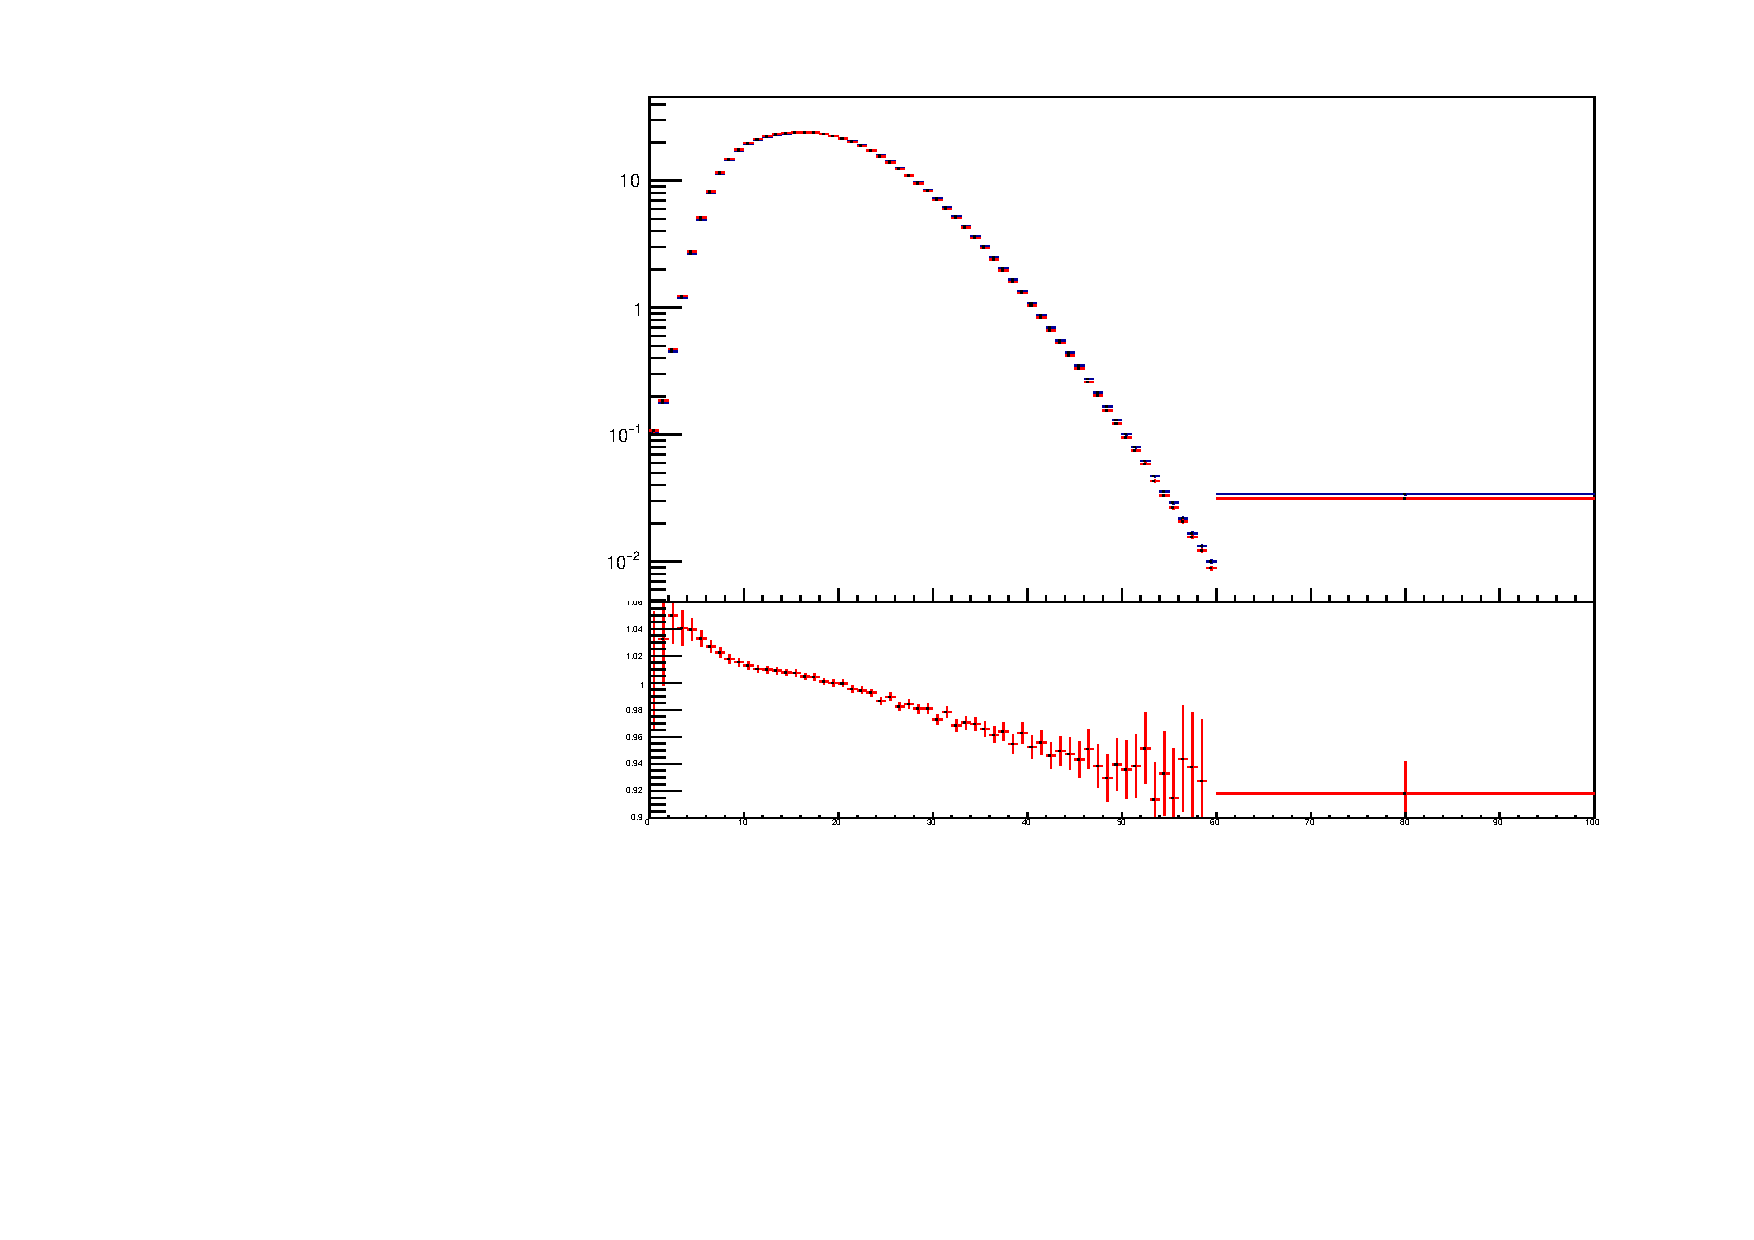
\includegraphics[width=0.48\columnwidth]{fig/Systematics/Tracking1.pdf}} 
%    \subfloat[]{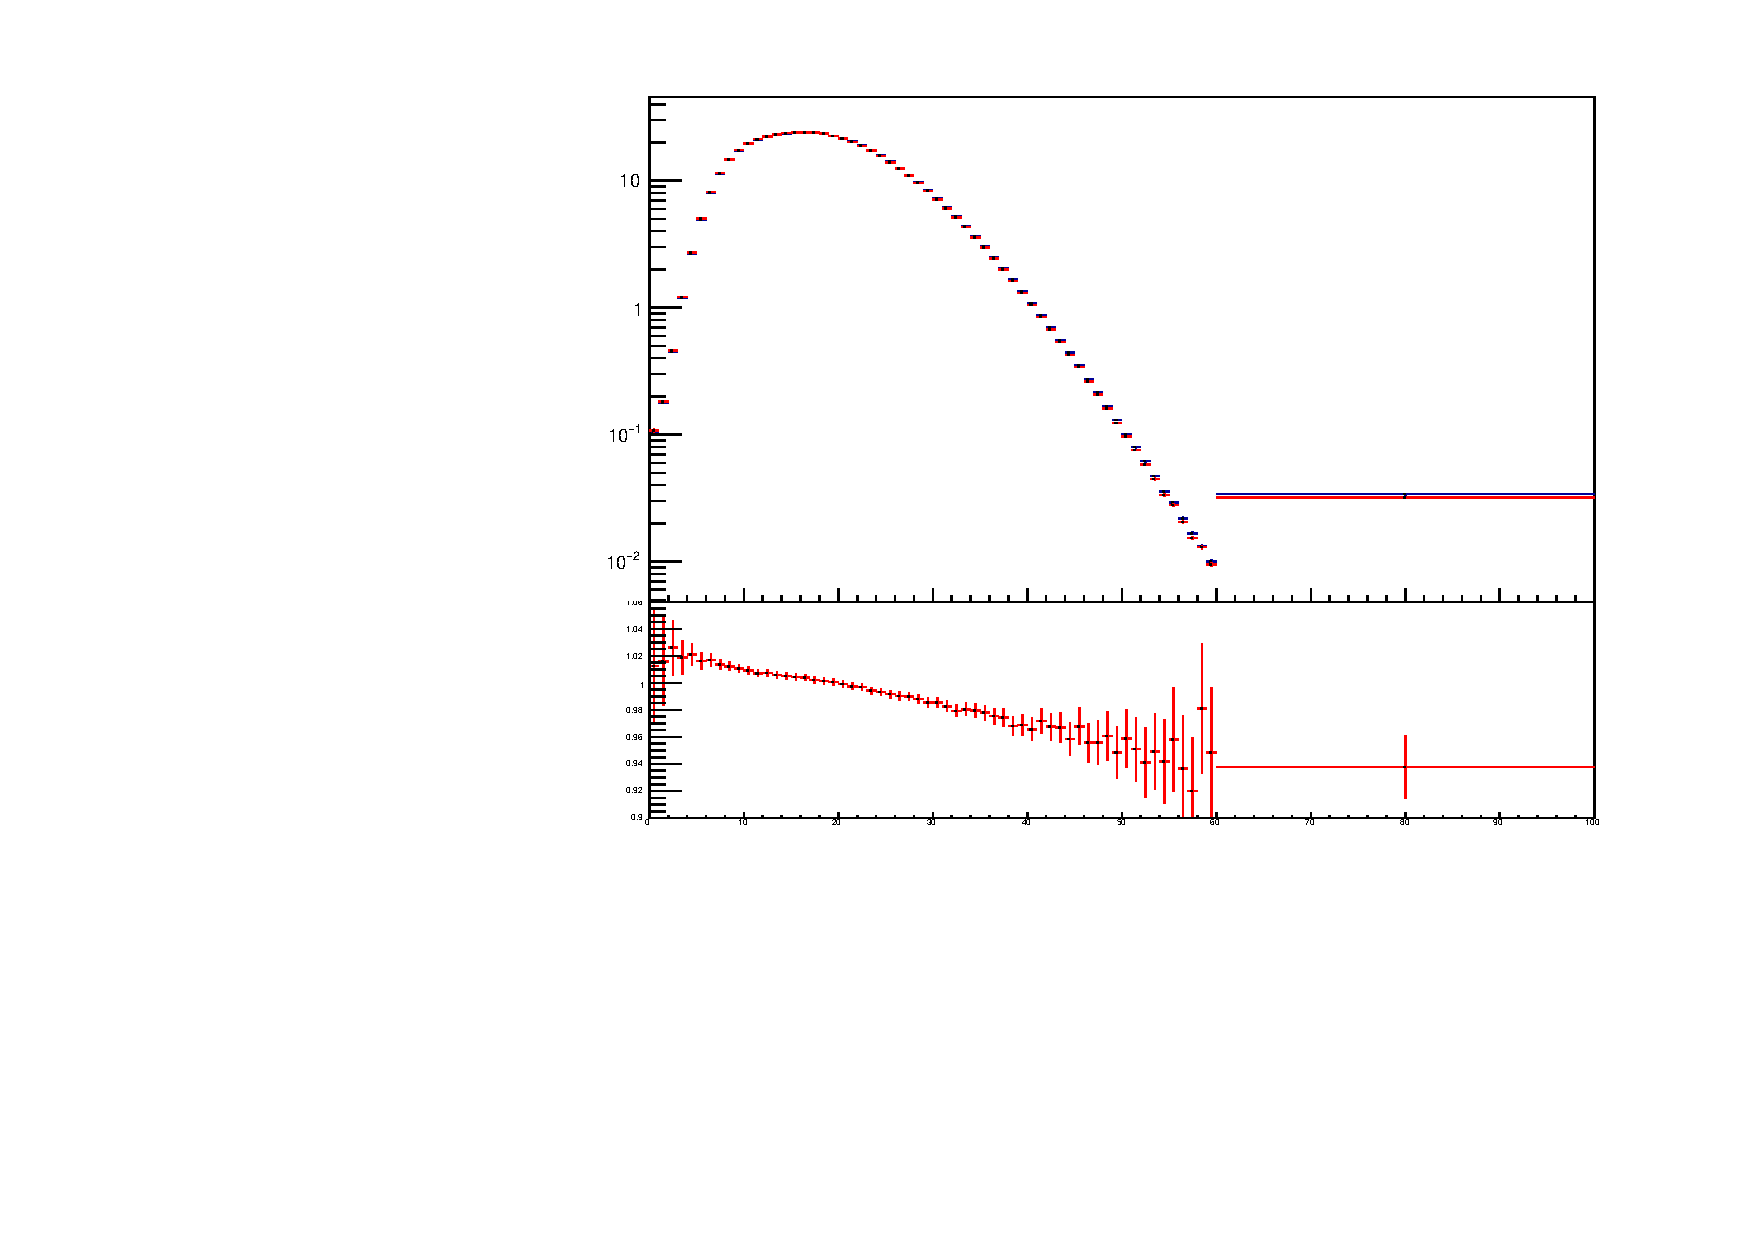
\includegraphics[width=0.48\columnwidth]{fig/Systematics/Tracking2.pdf}}   
%   \\
%    \subfloat[]{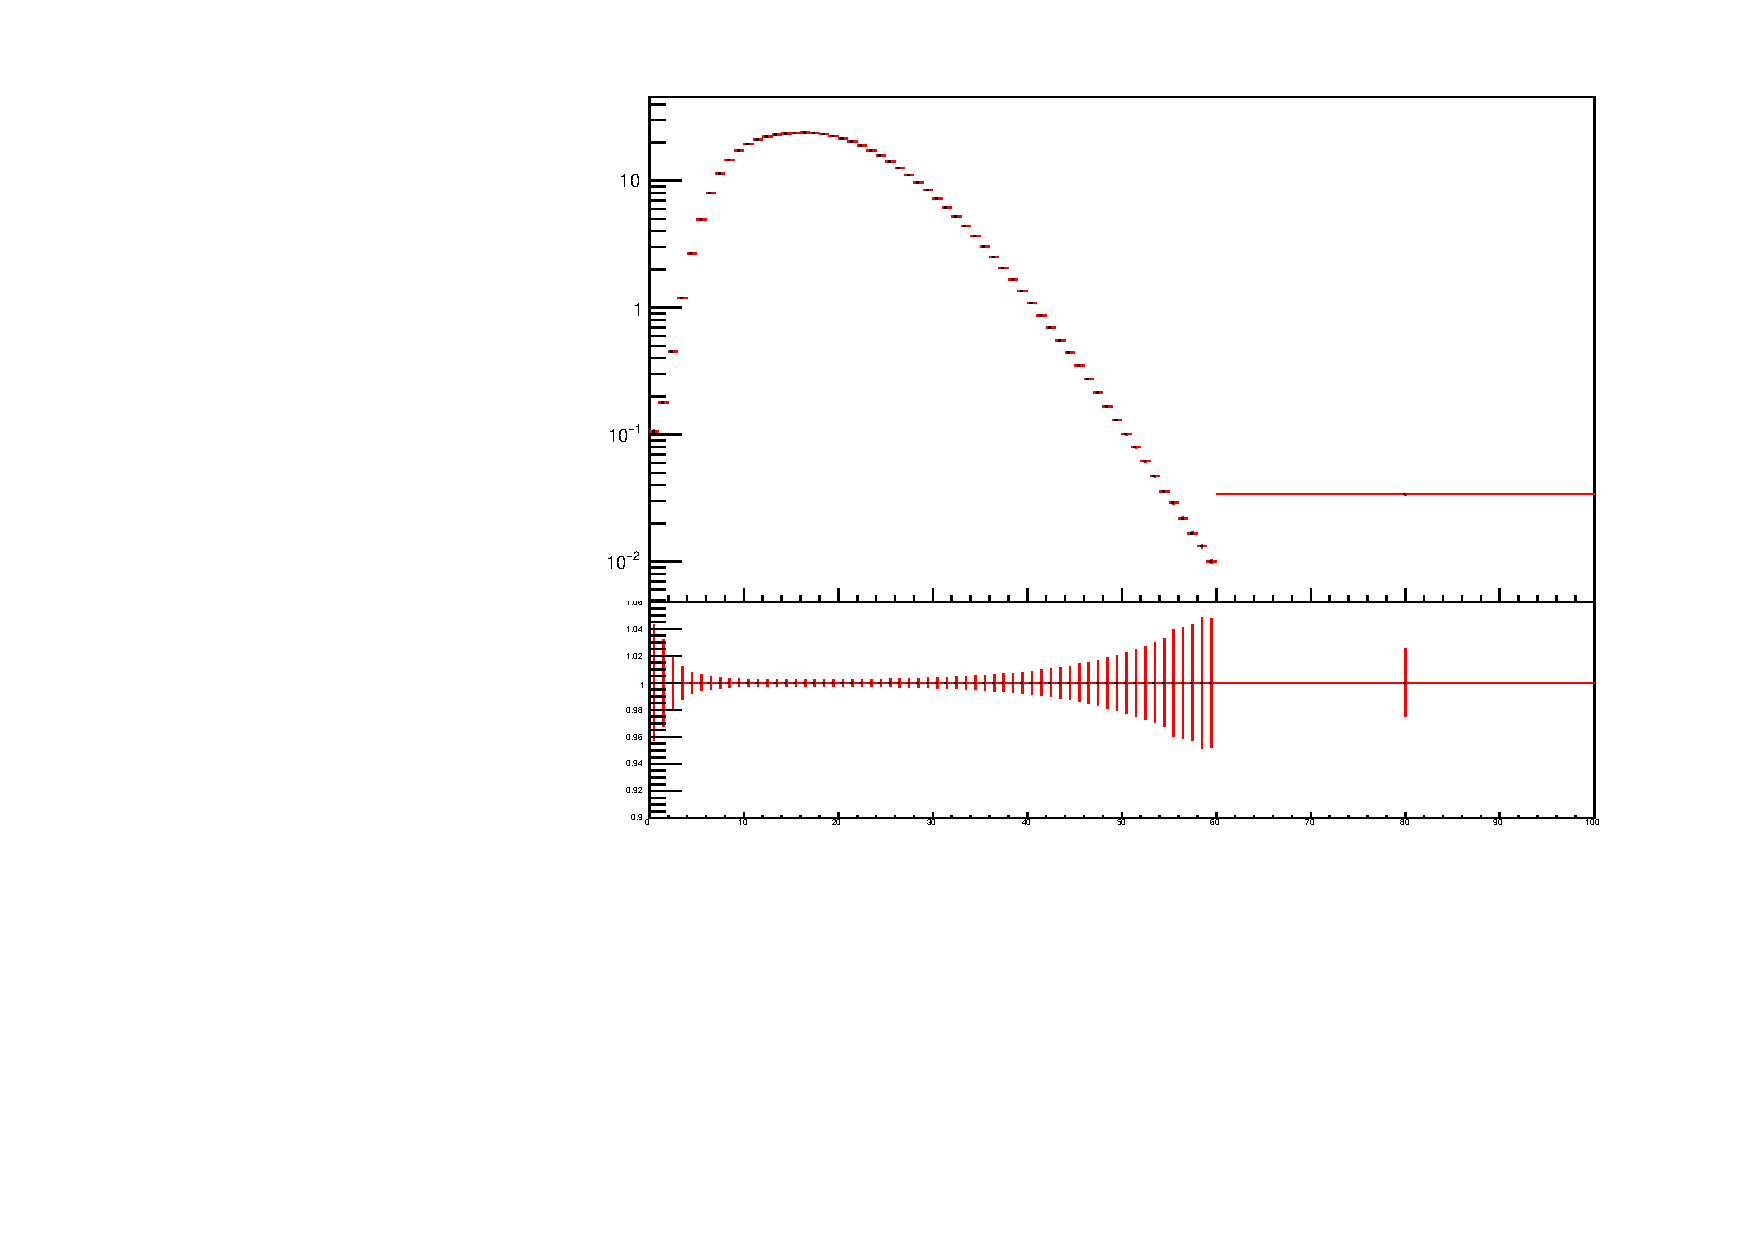
\includegraphics[width=0.48\columnwidth]{fig/Systematics/Tracking3.pdf}}
%    \subfloat[]{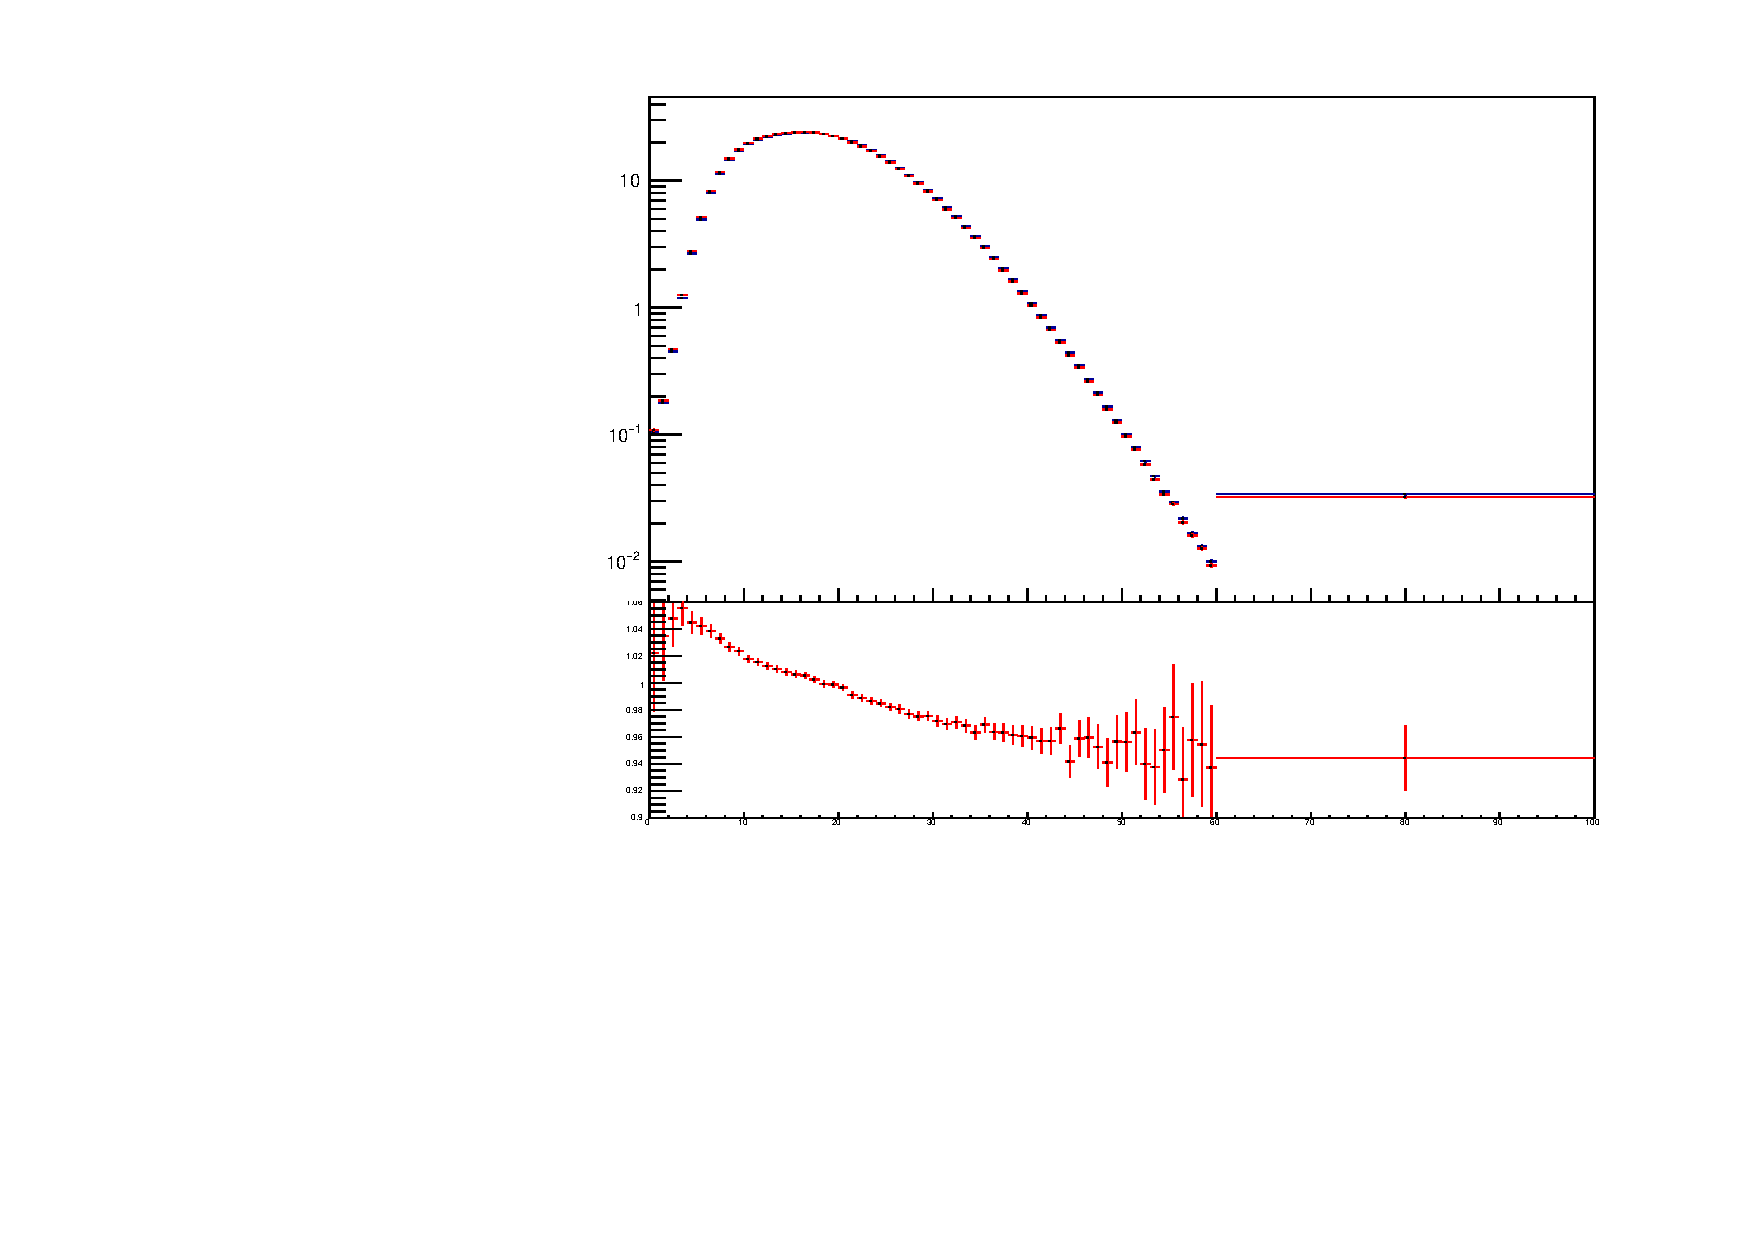
\includegraphics[width=0.48\columnwidth]{fig/Systematics/Tracking4.pdf}}     
%     \caption{Clockwise from left, the first plot shows the variation applied to account for track reconstruction efficiency. This is followed by the variation for the fake rate, the TIDE efficiency systematic and the uncertainty for weak modes in the detector alignment. As expected the variations (blue) from the nominal (red) are small, and in the case of the weak modes the effect is zero.}
%    \label{fig: ratioplots}
% \end{figure}
